\documentclass[a4paper,11pt]{article}
%\usepackage[T1]{fontenc}
\usepackage[utf8]{inputenc}
\usepackage[francais]{babel}
\usepackage{graphicx}
\usepackage{color}
\usepackage{cite}
\usepackage{algorithm}
\usepackage{listings}
\usepackage{listings}             % Include the listings-package
\lstset{language=c++}          % Set your language (you can change the language for each code-block optionally)
\usepackage{lstcustom}
\usepackage{amsmath}
\frenchbsetup{StandardLists=true} % à inclure si on utilise \usepackage[french]{babel}
\usepackage{enumitem}
\usepackage{amssymb}
\usepackage{algorithmic}

%pour les tableau
\usepackage{array}
\newcolumntype{M}[1]{>{\raggedright}m{#1}}

% nouveau symbole degré
\newcommand{\orto}{^{\circ}}

%-------------------------------------------------------------------------------
% Info Latex
%-------------------------------------------------------------------------------
%liaison bibtex : 
% REQUIRE IN CMD
% REQUIRE IN CORRECT Folder
%->latex spec
%->latex spec
%->bibtex spec
%->bibtex spec
%->latex spec
%->latex spec
% END 

%%%%%%%%%
% TITRE % Remplacer par un template spécifique
%%%%%%%%%
\author{Gagneux Julien}
%\title{
%\hfill \includegraphics[scale=0.7]{ifsttar.png}\\
%\hfill \includegraphics[scale=0.7]{p5.png}\\
%YATS :\\ 
%Yet Another Trafic Simulator \\ 
%Rapport de Stage\\
%\begin{large}
%du 18 Mars au 18 Septembre 2013
%\end{large}}

\begin{document}

\begin{titlepage}

\newcommand{\HRule}{\rule{\linewidth}{0.5mm}} % Defines a new command for the horizontal lines, change thickness here

\center % Center everything on the page

%----------------------------------------------------------------------------------------
%	HEADING SECTIONS
%----------------------------------------------------------------------------------------

\textsc{\LARGE Université Paris-Descartes }\\[1.5cm] % Name of your university/college
\textsc{\Large \textit{Institut Français des Sciences et Technologies des Transports et de l'Aménagement et des Réseaux}}\\[0.5cm] % Major heading such as course name
\textsc{\large Rapport de Stage}\\[0.5cm] % Minor heading such as course title

%----------------------------------------------------------------------------------------
%	TITLE SECTION
%----------------------------------------------------------------------------------------

\HRule \\[0.4cm]
{ \huge \bfseries YATS :\\
\vspace{0.5cm}
Yet Another Trafic Simulator}\\[0.4cm] % Title of your document
\HRule \\[4cm]
 
%----------------------------------------------------------------------------------------
%	AUTHOR SECTION
%----------------------------------------------------------------------------------------

\begin{minipage}{0.4\textwidth}
\begin{flushleft} \large
\emph{Auteur:}\\
Julien \textsc{Gagneux} % Your name
\end{flushleft}
\end{minipage}
~
\begin{minipage}{0.4\textwidth}
\begin{flushright} \large
\emph{Référent:} \\
Dr. Julien \textsc{Saunier} % Supervisor's Name
\end{flushright}
\end{minipage}\\[4cm]

% If you don't want a supervisor, uncomment the two lines below and remove the section above
%\Large \emph{Author:}\\
%John \textsc{Smith}\\[3cm] % Your name

%----------------------------------------------------------------------------------------
%	DATE SECTION
%----------------------------------------------------------------------------------------

{\large \today}\\[1cm] % Date, change the \today to a set date if you want to be precise

%----------------------------------------------------------------------------------------
%	LOGO SECTION
%----------------------------------------------------------------------------------------

\includegraphics[scale=0.8]{ifsttar.png}
\hfill \includegraphics[scale=0.7]{p5.png}\\

%\includegraphics[scale=0.7]{ifsttar.png}\\[1cm] % Include a department/university logo - this will require the graphicx package
 
%----------------------------------------------------------------------------------------

\vfill % Fill the rest of the page with whitespace

\end{titlepage}
%\maketitle %retirer apres l'ajout d'un template spécifique

% page de citation
\newpage

\vspace*{\fill} % insertion d'espace avant le text

\begin{large} % début d'agrandissement de la police 

\hfill Ces bricolages absurdes ne sont que des exercices, % replissage de blanc jusqu'au texte

\hfill mais comme on dit, pour arriver à l'intelligence artificielle,

\hfill il faut bien passer par l'imbécilité artificielle.\\

\end{large} % fin d'agrandissement de la police

\hfill \textbf{Hal Duncan}, 

\hfill \textit{ \underline{ Le Livre de Toutes les Heures } }, % italique + underline \uline marhce aussi 

\hfill tome 1 - page 198

%__________________________________________________________________________
% REMERCIEMENT 
%__________________________________________________________________________
\newpage
\section*{Remerciements.}
\addcontentsline{toc}{section}{remerciement}

\vspace{1cm}

\begin{large}

Rien n'aurait été possible sans la bienveillance et le soutient constant de Mr Julien Saunier : mon encadrant. Aussi mes premiers remerciement lui sont destinés sans aucune réserve. Merci d'avoir compris certaines de mes difficultés et de ne pas m'en avoir tenu rigueur, de m'avoir critiqué et soutenu dans mes démarches de recherches, mais surtout merci pour m'avoir choisi pour ces 6 mois, je résignerais sans hésitation. 

\vspace{1cm}

Je tiens aussi a remercier les doctorants Lancelot Six, Kevin Darty, Laurent Carafa ainsi que Abderraouf Zermane  pour m'avoir aidé a construire mon modèle.

\vspace{1cm}

Je souhaite également remercier Sophie Lemonier, Kevin Darty, Celine Mateev et Laurent Carafa pour leurs distractions bienvenues, les controverses que nous avons partagé lors de pauses clope interminables m'ont fait traverser se séjour au LEPSIS sur un petit nuage. J'espère que nous sommes un peut plus que des collègues.

\vspace{1cm}

Merci aussi à ma Mère, Patricia, d'avoir supporter la relecture de ce rapport sans rien connaitre ou presque à l'informatique et de me dispenser de si bon conseil depuis si longtemps.

\vspace{1cm}

Enfin je voudrais remercier Oriane. Celle qui supporte mes étranges lubies, celle pour qui j'ai envi de me lever le matin et avec qui se coucher le soir est toujours un grand bonheur.

\end{large}

\newpage

%__________________________________________________________________________
% Table des matières 
%__________________________________________________________________________
\newpage
%insertion de la table des matières
\tableofcontents
\newpage

%__________________________________________________________________________
% INTRODUCTION %
%__________________________________________________________________________
\section*{Introduction.}
\addcontentsline{toc}{section}{Introduction}

La Simulation Informatique offre des perspectives de recherche ainsi que des possibilités de prédiction étonnantes. Par essence la simulation est au réel ce qu'est un traducteur à une \oe{}uvre littéraire : un traitre.\footnote{"Traduttore, traditore", littéralement: "traducteur, traître", est une expression italienne. Cette expression est une paronomase qui joue sur la ressemblance des deux mots. elle est souvent utilisée même dans d’autres langues, en raison de la concision de ce jeu de mots.}

Elle trahit la réalité dans le sens où celle-ci est "\textit{tordue}" afin de convenir à un modèle lui même implémenté, donc lui aussi soumis à certaines lois comme le langage ou la plateforme sur lequel il est développé. Mais malgré ces entorses au réel, le développement d'un modèle est un moyen extrêmement efficace pour les chercheurs de comprendre plus en détail et plus en profondeur l'objet de leur recherche. 

Ici l'objet de nos recherches sera : "\textit{une modélisation agent des niveaux tactiques et opérationnels de la conduite, application au comportement latéral d'un véhicule}"\footnote{la fiche explicative du stage tel quelle à été diffusé se trouve en Annexe 1}. Ou, en raccourcissant : l'implémentation d'une nouvelle simulation de trafic : Yats. 

Nous approfondirons tout d'abord le contexte de ce stage dans la partie 1, nous présenterons notamment l'IFSTTAR (l'institut dans lequel j'ai eu la chance d'effectuer ce stage) et nous aborderons les cause et conséquence de la re-formulation de sujet du stage ce qui nous permettra de clairement préciser la problématique.

A la suite de cela, de la partie 2 nous verrons l'état de l'art actuel sur les simulateurs, la simulation, les systèmes multi-agents, les équations utilisées ainsi que certains concepts et définitions clés ayant orienté la conception du modèle.

Dans la troisième partie nous aborderons l'aspect pratique c'est à dire l'implémentation concrète du modèle théorique. Nous y verrons certaines fonctionnalité, les technologies utilisées, les subtilités de développement et les solutions mises en place. 

Certaines fonctionnalité ne peuvent être correctement décrit que dans une démarche pédagogique. Nous verrons donc dans la quatrième partie un manuel succinct d'utilisation, la présentation du benchmark et une biométrie légère de l'application.

Dans la cinquième et dernière partie de ce rapport nous nous intéresserons a ce qui pourrait être (ou qui sera) fait dans le futur; que ce soit le perfectionnement de certains objets et concepts ou encore la comparaison entre les trajectoires des véhicules de YATS avec des trajectoires de conducteur réel. 

Pour finir nous conclurons.

% 1 sujet
% 2 problèmatique 
% 3 plan 

\newpage

%__________________________________________________________________________
% CONTEXTE
%__________________________________________________________________________

\section{Contexte.}
\subsection{Présentation de l'ifsttar.}
J'ai eu la chance d'effectuer mon stage à l'IFSTTAR (\textit{Institut Français des Sciences et Technologies des Transports et de l'Aménagement et des Réseaux}). Cet établissement public placé sous la tutelle conjointe du \textit{Ministère de l'écologie, du Développement durable et de l'Energie}, et du \textit{Ministère de l'Enseignement Supérieur et de la Recherche}.

Le but de l'Ifsttar est de conduire des travaux de recherche et d'innovation dans le domaine des transports, des infrastructures et des risques urbains. 

Comprenant plus de 1200 agents \footnote{chiffres de 2011, source : http://www.ifsttar.fr/linstitut/colonne-1/lifsttar/quelques-chiffres-cles/} l'institut est composé de plusieurs départements, composés eux même des plusieurs laboratoire. Pour ma part je me suis joint au département COSYS (\textit{Composants et Systèmes}) dans le laboratoire LEPSIS (\textit{Laboratoire exploitation, perception, simulateurs et simulations}) ayant pour directeur : M Didier AUBERT.

Le LEPSIS mène des recherches dans trois domaines complémentaires a la limite entre ingénierie et science humaines : 
\begin{itemize}[label=-]
\vspace{-0.2cm}
\item Vision et Automatique Appliquées aux trajectoires,
\vspace{-0.2cm}
\item Systèmes Intelligents Appliqués aux Déplacement,
\vspace{-0.2cm}
\item Réalité Virtuelle appliquée aux simulateurs de conduite.
\end{itemize}
\vspace{-0.2cm}

Je fut placé sous la tutelle de Mr Julien SAUNIER, Docteur en Informatique, maitre de conférence à l'INSA-Rouen et chargé de recherche à l'IFSTTAR.

%Après un accueil chaleureux par l'équipe nous sommes rapidement rentré dans le vif du sujet.

\subsection{Redéfinition du sujet et problématique de recherche approfondi.}

Pour mieux cerner la problématique de ce stage nous allons commencer par dresser un petit historique du LEPSIS.

Il y a une vingtaine d'année fut développé le simulateur de conduite et de trafic :  ARCHISIM. L'initiative du projet fut lancé par M Stephane Espié au début des années 1990. Cela fait donc plus de 20 ans et durant ce temps les techniques de génie logiciel et les langages ont considérablement évolué. 

Archisim fut développé en Modula-2 \footnote{Langage de programmation créé en 1977 par Niklaus Wirth. Il est compilé, procédural, fortement typé et modulaire.}, langage dont l'apprentissage n'est pas très rependu. De plus Archisim fut développé majoritairement par des doctorants ou des stagiaires souhaitant en priorité affirmer (ou infirmer) leurs hypothèses. Ceci eu pour conséquence de ne pas avoir de réel suivi du projet en terme de version ou de procédure de test. Actuellement il est donc difficile de rentrer dans le code d'Archisim ce qui est un frein a la recherche. 

Il serait donc bienvenu d'avoir un logiciel plus léger, plus facile a appréhendé afin d'y tester certaines hypothèses sans pour autant avoir a apprendre un nouveau langage et rentrer dans une application complexe.

Avec le sujet de Mr saunier : Une modélisation agent des niveaux tactique et opérationnel de la conduite, en mettant l'accent sur le comportement latéral du véhicule, le sujet n'était pas uniquement de monter un modèle pour que le comportement latéral du véhicule soit plus cohérent avec la réalité mais également de produire un outil de prototypage.
\newline

En terme de recherche bibliographique la tache est importante. Chaque fonctionnalité de la simulation (par exemple l'accélération, le modèle multi-agent, etc..) a fait l'objet de nombreuses recherches et publication. Il m'aura fallu lire des dizaines d'articles et parler de nombreuses heures avec les chercheurs du LEPSIS avant de commencer à cerner le sujet. 

En ce qui concerne l'implémentation, la technique pure, la aussi les choix du langage et des bibliothèques orienta fortement la manière de concevoir la plateforme et la mise en œuvre du le modèle.

Bien sur développer un logiciel implique forcément de développer certaines spécifications extra-fonctionnelles (ou fonctionnalités pour la plateforme et non pour le modèle), nécessaires mais chronophages, comme la gestion des logs ou le développement de réseau routier.\\

Finalement ce qui devait être une étude sur le la modélisation du comportement latéral du véhicule se transforme en un développement d'envergure d'une application pour développeur et chercheur nommé : "YATS" \footnote{ Acronyme de : "Yet Another Trafic Simulator"} qui permettra par la suite de concevoir des modèles répondant a de nombreuse question, dont celle initialement prévu pour ce stage. 

\newpage

%__________________________________________________________________________
% ETAT DE L'ART et MODELE THéORIQUE
%__________________________________________________________________________

\section{État de l'art et modèle théorique.}

Nous aborderons dans cette partie les concept théoriques clés afin de bien comprendre les choix techniques de la partie 3. Nous justifierons nos choix par une bibliographique concise. 

Le choix du type de simulation s'est immédiatement orienté vers un système multi-agent. Seulement concevoir un SMA repose sur un paradigme en développement n'ayant pas encore fait concrètement ses preuves dans le secteur privé ou dans l'industrie comme l'a fait le paradigme objet. Il est des lors facile de tomber dans des pièges que seule l'expérience permet d'éviter, d'où une étude approfondi de la littérature sur le sujet. Cependant nous resterons succin dans nos définition.

Débutons par la définition d'un Agent.

\subsection{Agent intelligent.}
Il est difficile de trouver dans la littérature scientifique une définition pour définir ce qu'est un agent intelligent et de faire l'unanimité parmi les chercheurs. Nous resterons donc classique en donnant une définition généraliste de Wooldrige et Jennings \cite{jennings1998agent} : \\

\fbox{\parbox{0.90\textwidth}{"Un \emph{agent} est un système informatique situé dans un \emph{environnement}, étant capable \emph{d'actions autonomes} dans le but des réaliser les objectifs pour le(s)quel(s) il à été conçut."}}\\

De cette définitions découle quelques propriétés : 
\begin{itemize}
  \item Si un agent vie dans un environnement il est donc \textbf{situé}.
  \item Il prend ses propres décision : il est donc \textbf{Autonome}.
  \item Il \textit{vie} dans le but de réaliser ses objectifs personnels.
\end{itemize}

Cependant il manque une part importante de ce qui constitue l'agent : \textbf{la rationalité}. Prenons par exemple un agent stupide ayant pour but de rejoindre un point quelconque. Cet agent à le choix entre plusieurs chemin mais celui-ci prend la décision de tourner à droite à chaque intersection. Nul doute que cette agent risque de tourner en rond longtemps. Dès lors, et c'est en quelque sorte l'un des but de l'intelligence artificielle : un agent se doit d'être rationnel pour en porter le nom. Bratman \cite{AICPub540:1988} et \cite{bratman1987intention}

\subsection{L'encorporation de l'agent.}
%a reviser minimum 50 fois !

Cette partie touche plusieurs matières scientifique et est donc sujet a de grandes controverses. L'aborder reste cependant fondamentale pour le domaine de l'intelligence artificielle, mais aussi parce qu'elle a orienté la conception du modèle. 

A l'origine des ses questionnement se trouve l'ouvrage des professeurs Pitti et Pfeiffer \cite{pitti:hal-00763867}. Ce livre propose de changer un peut notre vision de l'agent en tant qu'entitée logique pur et dur. Ils avancent le fait que l'encorporation de l'agent (le fais que l'agent aie un corps à lui) physique (pour le cas des robots) ou virtuel (pour le cas des simulations) change les rapports qu'entretient l'agent avec le monde et lui même. 

Ceci implique de très nombreuses réflexions, notamment celle de l'apprentissage. Nous (en tant qu'agent intelligent et rationnel) avons appris à utiliser notre corps. Notre cerveau (notre artefact de la décision) à lui aussi appris à force d'innombrable répétions les conséquences physiques de nos actions sur le monde.  Changez de corps et toutes ces perceptions et influes devront être adaptés et réappris. 

Pourtant, et a l'insu de nos propres choix formulé rationnellement par notre cerveau, nôtre corps prends en permanence ses propres décision. Pitti \& pfeifer avancent ici qu'en fin de compte si fiers de nos décisions, nous en oublions que beaucoup sont prises par notre corps, sans que l'on soit finalement consulté. 

Un exemple : songez à vôtre pas. Vous marchez juste calmement dans la rue. Nul doute que vous avez pris la décision d'aller quelque part initialement, cependant pensez vous à chacun des éléments de décision que nécessite la marche ? Je ne pense pas mais soyons rigide et admettons que nous pouvons en effet segmenter la marche en une suite d'actes simple. 

Lever la jambe $\rightarrow$ plier le genoux $\rightarrow$ poser le talon $\rightarrow$ transférer le poids sur l'autre pied $\rightarrow$ etc.. 

Néanmoins, avez vous conscience que vos muscle se détendent lors de la descente de votre pieds vers le sol en utilisant la gravité de la terre afin de faire moins d'effort ? Personne sur terre ne pense à cela à chaque pas effectué, et heureusement car notre tête exploserait littéralement sous la somme des calculs qu'il serait nécessaire de faire. C'est dans ce sens la que Pitti \& pfeifer propose de repenser l'encorporation de l'agent. 

Avec un corps c'est énormément de processus de bas niveau qui se doivent d'être automatiser, par l'apprentissage ou par quel-qu'autres moyens. l'obtention, ou la conceptions d'un corps propulse l'agent à un niveau de rationalité bien supérieur étant donné qu'il n'a qu'a se focaliser exclusivement sur les taches de réflexions et/où de décision.

La porté philosophique de cette hypothèse est tellement large que nous n'en débattrons pas ici. Recentrons nous donc sur notre simulateur de trafic. Le but ici est de pouvoir changer de corps suivant les paramètres. Par changer de corps nous n'entendons pas changer de corps en cours de simulation évidement, mais qu'a chacune des sources (nous y reviendrons) faisant naitre des véhicules, ceux-ci puissent avoir des caractéristique et des méthodes différentes. 

Car au final c'est cela un corps : un ensemble d'attributs et de méthodes propres.

\subsection{SMA}

Un SMA (Systeme Multi Agent ou MAS : \textit{Multi Agent System} en anglais) se distingue d'un système informatique classique par bien des aspects. selon Draa \cite{Draa2001} un SMA se distingue d'un programme classique dans la mesure ou il n'y a pas de contrôle global du SMA. 

Chaque agent est un fragment du système global et rempli sa tache qui est une sous tâche de la tâche global. 

Un SMA est donc composé d'entités artificielles intelligentes : les agents. 

Ces agents évoluent dans un environnement dont ils font partie intégrant (nous reviendrons sur l'environnement par la suite). 

Ces agents se doivent d'avoir des interactions entre eux dans le sens ou les agents seront mis en relation pour l'accomplissement de leur tâche, et Cela même dans le cas d'agents "autistes".

Un groupe d'agents (même petit) est par définition une société avec son organisation et ses règles. \\

Nous venons de voir ici une liste succincte des principales caractéristique d'un SMA. Pourtant ce que nous désirons construire est un logiciel de simulation qui lui aussi répond a des caractéristiques précises.

\subsection{Simulation et Développement itératif.}

Nous touchons ici a un sujet extrêmement sensible doté d'une littérature très abondante. Commençons par définir ce qu'est une simulation.

La première définition fut celle de Shanon (1976) \cite{Shannon:1977:SMM:1102766.1102770} qui désigne la simulation comme : \\

\fbox{\parbox{0.90\textwidth}{ 
Un processus dont le point de départ est de concevoir un modèle a partir d'un system réel.}}\\ 

Ceci met en lumière 2 concepts clés : le système réel (que l'on cherche a reproduire artificiellement) et le modèle (l'implémentation du système réel). 

Cela nous amène a la définition proposé par Fiswick (1994) \cite{Fishwick94computersimulation:} pour qui : \\

\fbox{\parbox{0.90\textwidth}{ 
La simulation est un processus de conception itératif, cyclique et non-linéaire dont le point central est le modèle réalisé a partir d'un système. }}\\

Le schéma ci-dessous (aussi extrait de \cite{Fishwick94computersimulation:} ) illustre parfaitement cette définition. 

\begin{center} \includegraphics[scale=0.7]{SimConception.PNG} \end{center}

Nous remarquons donc que créer une simulation apparait plus compliqué qu'il n'y parait au premier abort. 

Reformulons : nous souhaitons réaliser un logiciel d'un type particulier (une simulation) dont le développement engendre une technique de développement particulière (un développement itératif). 

Le cycle itératif offre plusieurs avantages notamment la stabilité du projet et une meilleurs gestion des risques. Cependant ce type de modèle de développement présente aussi des inconvénients comme sa lenteur (surtout à causes de la masse de test a effectuer à chaque itération). De plus comme nous sommes dans le cadre du développement d'une simulation le modèle en lui même n'est pas totalement défini et il y a de grande chance que le cycle "$n$" doive être complètement réécrit car incompatible avec la l'élaboration du cycle "$n + X$".

Nous pouvons, a titre informatif lister l'ensemble des cycles traversés durant ces 6 mois de stage : 

\begin{enumerate}[label=-]
\item 
Phase préliminaire : Reformulation du sujet - apprentissage des technologies - maquette.

\item 
Cycle 1 : essais de véhicule respectant approximativement la physique 2D de base.

\item 
Cycle 2 : essais de route et manipulation de la SDL.

\item 
Cycle 3 : élaboration approfondie - Développement des fichiers source externes puis d'une technique de développement du réseau routier.
 
\item
Cycle 4 : développement d'un comportement réaliste des Véhicules/Agents. Accélération, ralentissement et virage.

\item
Cycle 6 : Approfondissement des fonctionnalités graphiques. déplacement, homothétie.

\item
Cycle 7 : Approfondissement des fonctionnalités des Sources 

\end{enumerate}

Nous reviendrons sur beaucoup des points lister ci-dessus mais ce qu'il est important de garder à l'esprit c'est que développer une simulation nécessite la mise en place de procédure de développement spécifiques rigides si l'on ne veut pas se retrouver avec un système instable avec de erreurs impossible a résoudre a l'itération suivante. 

Il est important de dire aussi que j'ai "naturellement" adopter un cycle itératif et que la découverte d'une technique de développement propre aux simulations est arrivé milieu fin de stage.

Continuons maintenant de décrire les concepts théoriques qui on orientés le développement de YATS.

\subsection{Un rapport stigmergique avec le monde.}

Tout d'abord définissons ce qu'est la stigmergie :\\

\fbox{\parbox{0.90\textwidth}{ 
La stigmergie est une méthode de communication indirecte dans un environnement émergent auto-organisé, où les individus communiquent entre eux en modifiant leur environnement. \cite{Dorigo:2000:AAS:348599.348601} et \cite{Weyns05environmentfor}. }}\\

Les fourmis sont un parfait exemple pour illustrer ce qu'est concrètement la stigmergie. Lorsque celles-ci se déplacent elles déposent des phéromones afin d'indiquer où elles sont passées. Les autres fourmis, lorsqu'elles voudront emprunter ce même chemin s'apercevront qu'une autre fourmi est déjà passé par là car elle a modifié sont environnement et cette modification a été perçu. Les deux fourmis ont donc bien communiqué les unes avec les autres de manière indirecte en modifiant leur environnement. 

Dans le cadre de notre simulation de trafic cette notion apparait comme fondamentale, les véhicules ne pouvant évidement pas communiqué directement en utilisant des requêtes personnelles, ceux-ci devront modifier leur environnement.

Nous pouvons noté que lors de l'exercice de la conduite (dans la réalité et par des humains donc) c'est exactement ce qui se produit. Les conducteurs ne discutent pas ni pour obtenir des informations, ni pour prendre des décision et cela même à l'arrêt. Lorsqu'un conducteur va tourner à gauche celui-ci modifie l'environnement en plaçant une balise visuelle clignotante lumineuse de couleur orangé sur le  coté gauche de son véhicule. Les autres conducteurs perçoivent cette balise et en interprète l'information : "-ce conducteur va tourner à gauche". les conducteurs se sont transmis une information à l'aide de l'environnement sans pour autant qu'il y ai eu de requête directe.

Dans notre simulation de trafic nous appellerons ces balise des \textbf{tags} \cite{Platon2005}.

\subsection{Environnement.}

l'environnement est l'un des élément central d'une simulation basé sur un système multi-agents. Seulement comment le construire ? quel sont les propriété qu'il doit posséder ou ne pas posséder ? quel sont les erreurs a éviter ? 

A ma connaissance il n'existe pas de "manuel de développement de l'environnement idéal". Nous baserons donc nos réflexions sur trois document de références de Weyns : 2005\cite{Weyns05environmentfor} 2006\cite{conf/e4mas/WeynsH06} et 2007\cite{env-jaamas14} 

Nous pouvons déjà distinguer deux perspectives d'environnement :
\begin{enumerate}[label=-]
\vspace{-0.25cm}
\item l'environnement pour un system d'agent situer; c'est celui qui va nous intéresser
\vspace{-0.25cm}
\item l'environnement pour un system d'agent cognitif; dans ce cas, si nous pouvons nous permettre une comparaison il représente un conteneur favorisant les actions de l'agent (ex: communication, taches externes, etc..).
\vspace{-0.25cm}
\end{enumerate} 

Dans le cas de l'environnement pour des agents situés, celui-ci doit pouvoir permettre de faire des \textit{actions situées}. Cela nous concerne tout particulièrement pour notre simulation de trafic ou lorsqu'un Agent tourne à gauche il le fait localement. L'Agent évolue donc dans un \textit{monde externe} a part entière.

Nous avons parlé un peut avant de stigmergeie dans lequel l'environnement joue le rôle de moyen de coordination et de communication. C'est donc un élément central du projet. 

Nous venons de survoler ce qui devrait composer l'environnement. Nous prendrons comme référence La Definition que donne Weyns dans \cite{conf/e4mas/WeynsH06} (non traduit pour dénaturer le moins possible le sens) :
\\

\fbox{\parbox{0.90\textwidth}{"The environment is a first-class abstraction that provides the surrounding conditions for agents to exist and that mediates both the interaction among agents and the access to resources."}}\\ 

\vspace{0.25cm}

Cette définition implique beaucoup de chose, notamment que l'environnement est essentiel pour l'existence de l'agent. Il structure sa vision du "monde", ses échanges et les actions qu'il permet ou nom de faire. Il est en quelques sorte le garant de la cohésion \textit{"sociale"} et \textit{"physique"} du système.

Nous pouvons dégager de cela trois façon pour l'Agent d'interagir avec l'environnement : 

\begin{enumerate}[label=-]
\vspace{-0.25cm}
\item \textbf{Perception} : l'Agent perçoit localement son environnement.
\vspace{-0.25cm}
\item \textbf{Action} : l'Agent peut exercer des actions sur l'environnement.
\vspace{-0.25cm}
\item \textbf{communication} : l'Agent communique avec les autres agents par le biais de l'environnement. 
\vspace{-0.25cm}
\end{enumerate}

L'environnement est donc un véritable support pour le système multi-agents.

\subsection{Affordance.}

Ce concept : l'affordance, a largement influencé la conception du modèle de notre simulateur. Ce concept fut développer initialement par le psychologue James J. Gibson\cite{Norman:1999:ACD:301153.301168} en 1977 et a été repris par le suite par de nombreux chercheur dans de nombreuse matière, notamment en ergonomie

définition de l'affordance :\\

\fbox{\parbox{0.90\textwidth}{L'affordance est la capacité d’un système ou d'un produit à suggérer sa propre utilisation.\footnote{http://fr.wikipedia.org/wiki/Affordance}}}\\ 

Étant donné que dans notre modèle, qui orienté SMA, les agents vont utilisé des objets de leur environnement, ces objets se doivent d'avoir une utilisation "ergonomique". Nous reviendrons sur un exemple d'utilisation du concept d'affordance dans la partie pratique.

\subsection{Mathématiques élémentaires}

Yats peut se définir en quelques sorte comme un cas concret d'utilisation des concepts mathématiques de base. les références dans les code y sont fait en permanence que ce soit dans les procédures de décision, d'application des éléments physique ou encore de l'affichage.

Nous allons commencer au plus bas niveau de l'algèbre linéaire en passant par la trigonométrie et les espaces vectoriels. Nous verrons enfin un problème physique concret : l'accélération. 

\subsubsection{Algèbre linéaire}

\begin{enumerate}[label=-]
\item 
L'équation d'une droite dans un plan se présente sous la forme : 

$ y=ax+b $

\item 
Lorsque nous n'avons que deux points pour déterminer l'équation d'une droite : 

\begin{enumerate}[label=.]
\item PA($x_a , y_a$)
\item PA($x_b , y_b$)
\end{enumerate}


$ a = \dfrac{y_b-y_a}{x_b-x_a} $ 

$ b = y_a - (a*x_a) $

\item
Lorsque nous devons déterminer la distance cartésienne (à vol d'oiseau) entre deux points \\

$ \sqrt{(x_b-x_a)^2 + (y_b-y_a)^2 } $

\end{enumerate}

\subsubsection{Trigonométrie et espace vectoriel}

\begin{enumerate}[label=-]

\item 
Lorsque nous n'avons qu'un point et un angle pour déterminer l'équation d'une droite nous allons devoir utiliser le cercle trigonométrique : 

\includegraphics[width=0.55\textwidth]{cercletrigo.PNG}\\

Il y a bien sur énormément de choses a dire sur ce schéma mais le plus important à retenir ici est que : \\

$ \vec{OM} = \cos( \alpha ) \vec{OI} 
		   + \sin( \alpha ) \vec{OJ}     $\\
		   
nous allons nous servir de ceci pour projeter un point $P(x_1;y_1)$ à l'emplacement voulu selon l'angle $\alpha$ (en degré) sur une distance $(\vec{OM})$\\

$ x_2 = x_1 + ( \vec{OM} * \cos(\alpha * \dfrac{\pi}{180})) $ 

$ y_2 = y_1 + ( \vec{OM} * \sin(\alpha * \dfrac{\pi}{180})) $ \\

\item 
Déterminer l'angle $\beta$ d'une droite par rapport a l'axe des abscisses : \\

$ \beta = - \arctan (pente) * \dfrac{180}{\pi} $ \\


\item
Pour déterminer l'angle entre deux droites :

Étant donné deux droite dont nous pouvons connaitre l'angle par rapport a l'axe des abscisses :  \\

$ diff(\beta_{d1},\beta_{d2}) $\\

En pratique cela implique quelques subtilités algorithmiques qu'il n'est pas nécessaire de développer ici.

\end{enumerate}

\subsubsection{Homothétie et espace vectoriel}

	Zoomer ou Dé-zoomer revient concrètement a changer d'échelles. 
	
	En géométrie nous parlons d'homothétie dans un espace affine% citer le bon auteur
, c'est à dire que pour tout les points "P" de notre repère et selon le centre "O" et de rapport "r" (non nul) nous avons $\vec{OP} = r*\vec{OP}$

l'image ci-dessous exprime très simplement se concept.\newline

\begin{center}
\includegraphics[scale=0.8]{Homothetie.png} \\
\end{center}

Nous pouvons très simplement mettre en place cette formule par : \\

pour un point : $ P(x_p, y_p) $

pour un point d'Origine (ici le curseur de la souris) : $ O(x_o, y_o) $

pour un facteur : $ r $\\

$ x_p = r * (x_p - o_x) + o_x $\\

$ y_p = r * (x_y - o_y) + o_y $\\

\subsubsection{Accélération}

Réussir à trouver une formule crédible pour l'accélération et la décélération (qui est aussi une accélération négative) fut un des plus gros challenge de ce projet. Certains passent une thèse à y réfléchir, ici nous n'avions pas ce luxe.

Plus encore, déterminer un moyen de faire avancer un véhicule de manière crédible n'étant pas une fonctionnalité principale du projet il fallut la réaliser rapidement. Mais après la lecture d'innombrable article peut stimulant j'ai été chercher de l'aide, j'avais avant tout besoin d'inspiration. Tout ceci fut débloqué grâce au léger coup de pouce de Mr Roland BREMOND, chercheur au LEPSIS, après avoir discuté d'une unité de mesure : le mettre par seconde carré, ou ms$^2$. C'était finalement si simple.\\

reprenons la problématique de cette partie : nous voulons que nos véhicules avance et freine de façon crédible. 

concrètement, l'accélération correspond à la variation de la vitesse entre deux mesures de temps. nous pourrions aussi noter cela ainsi : \\

$ a = \dfrac{\delta_v}{\delta_t} $\\

Où $ a $ est l'accélération, $ v $ est la vitesse et $ t $ est le temps (nous reviendrons sur le temps dans la partie 3 : "implémentation").

Ce qui nous intéresse tout particulièrement ce n'est pas d'avoir la formule ultime, mais bien de connaitre la position de notre véhicule après un pas de temps. Et pour cela aussi il y a une formule : celle de la distance parcourue en fonction d'une durée : \\ 

$ d = d_0 + v_0\delta_t + \dfrac{a\delta_t^2}{2} $\\

$ d_0 $ représente le déplacement initial, $ v_0 $ la vitesse initiale, $ \Delta_t$ la durée du trajet et $ a $ l'accélération

Que nous restait-il à faire ? Déterminer la valeur de a. La encore c'est Mr BREMOND Roland qui nous indiqua le chiffre d'or : 5.

Il est cependant intéressante de savoir que a dans la plupart des cas ou cette formule est utilisé, $ a $ vaut 9,81, soit la valeur de la gravité.

La formule que nous avons donc utilisé est très proche de celle de la distance parcouru par un solide dans l'espace pour un temps donné. Ce qui n'est au final pas surprenant.

L'implémentation de la formules est beaucoup plus facile a comprendre que la formule, même si ce n'est pas exactement sous cette forme qu'elle apparait dans le source de l'application. \\

\begin{lstlisting}[language=c++, style=eclipse, frame=single]   

        // frequence d'echantillonage en secondes
    const double dt = 0.5;     	
    const double accel = 9.81; // m/s carre
    double speed = 0.0;        // m/s
    double position = 0.0;     // m
    double time;
    for (time = 0.0; time < 2.5; time += dt){// end at 2.5s
        position += (accel * dt * dt / 2.0) + speed * dt;
        speed += accel * dt;} 
\end{lstlisting}

\vspace{0.25cm}

Avec ce segment de code nous allons basculer de chapitre et passer a l'implémentation du projet.

\newpage

%_______________________________________________________________________________
% PARTIE 3 : IMPLEMENTATION 
%_______________________________________________________________________________
\section{Implementation.}

Avec ce chapitre nous allons nous confronter a des problématiques bien plus concrète Comme le choix des technologies ou l'architecture mis en place.

\subsection{Résumé schématique.}

Le Schéma ci-dessous nous fourni une vision simpliste mais réaliste de ce qui a voulu être construit. 

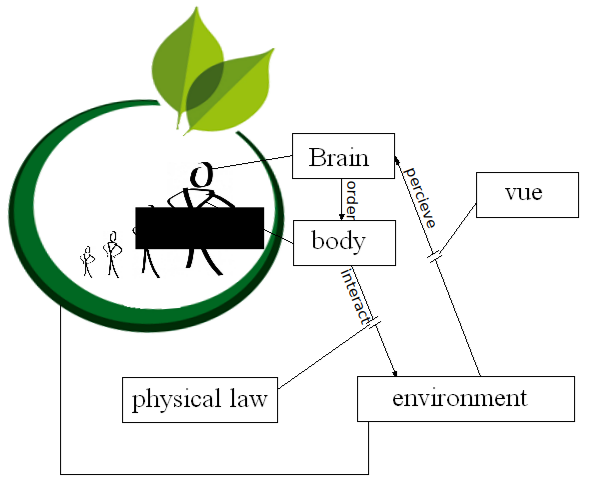
\includegraphics[width=\textwidth]{ModelConcetuel.PNG}
% faire attention aux majuscules dans le shcéma. 
% rétablir ou généralisé l'erreur de "B"rain

Nous sommes dans le cadre d'un système multi-Agent. Chaque Agent est composé d'un \textit{Brain} comme entité logique et d'un \textit{Body} afin de pouvoir changer de véhicule dans le futur, par exemple utiliser des camion au lieu de voiture, changer la taille des voiture, etc.

L'agent interagi avec l'environnement dans lequel il doit respecter les lois physiques. 

Afin d'augmenter le réalisme et comme il est clairement stipulé dans l'article de Weyns \cite{Weyns05environmentfor}, il serait vue comme une erreur d'envoyer tout l'environnement en argument brute à l'agent. Nous avons donc créer une Vue qui correspond a un sous ensemble d'information provenant de l'environnement. L'agent perçoit sont environnement localement grâce a cette vue. 

\subsection{Choix et description des technologies utilisés.}

Dans cette sous partie nous allons voir rapidement le langage que nous avons utilisé, dans quel environnement de développement et avec quelle bibliothèque.

\subsubsection{Language.}

L'un des but énoncé dans la partie 1.2 était de pouvoir appréhender plus facilement le code pour les chercheurs du LEPSIS. Pour cela il y a un moyen assez simple : utilisé un langage que tout le monde connait. Nous avons donc choisi le C++. 

Beaucoup de monde connait le célèbre langage développer par Bjarne Stroustrup\footnote{Est-il vraiment nécessaire de présenter Bjarne Stroustrup ? Écrivain et professeur des Sciences Informatiques Danois. Inventeur notamment du langage C++.}, de plus il permet un développement d'une extrême finesse, des performances ainsi qu'une gestion de la mémoire optimale.

\subsubsection{IDE.}

Après quelques essais et difficulté nous avons opté pour Microsoft Visual C++ Express Édition car nous bénéficions d'une meilleur expertise de base sous cette IDE.

Il n'y a pas grand chose à dire de plus sur l'IDE, passons rapidement aux bibliothèques que nous avons utilisé. 

\subsubsection{Bibliothèques.}

Évidement nous avons utilisé quelques une des classes de la STL.

Cependant il nous fallait représenter graphiquement nos véhicules et leur mouvements. Ceci offre plusieurs avantage, par exemple de pouvoir contrôler visuellement leur déplacement ou vérifier la fiabilité instinctive que nous avons du modèle.

Après quelques discussion nous avons opté pour la SDL.

\includegraphics[scale=0.25]{SDL_logo.PNG}

SDL est l'acronyme de "Simple DirectMedia Layer". C'est une bibliothèque Cross-Platform permettant un accès bas niveau au son, clavier, souris, et dispositif d'affichage comme les écrans.

C'est une bibliothèque très performant ayant largement fait ses preuves, notamment grâce aux jeux vidéo\footnote{pour ne citer qu'un seul exemple célèbre : mario fut développer en SDL.}. Elle nous permettra de manipuler des Surface (ensemble de pixels rectangulaire à l'écran). Et c'est tout...

SDL est une bibliothèque très bas niveau ce qui implique qu'elle est développer en C. Son encapsulation dans des classe doit donc veiller au strict respect de l'ordre des appels des fonctions de base.

Certaines fonctionnalités que nous voulions développer n'était pas initialement possible avec la SDL. Nous avions donc deux choix. Soit redevelopper les fonctions qui nous intéressaient soit aller piocher dans les SDL\_XXX. Ces bibliothèque fonctionne en annexe de la SDL par exemple SDL\_ttf permet de manipuler du texte dans les images.

Nous avions besoin de deux éléments supplémentaire. Tout d'abord pouvoir faire des rotation de surface et des zoom. Nous avons donc rajouter au projet la bibliothèque SDL\_GFX. Celle-ci inclue l'objet RotoZoom\_Surface qui permet, comme son nom l'indique, de faire des rotations et des zooms.

Nous avions aussi Besoin de faire des formes qui ne soit par rectangulaire : des ronds. SDL\_Draw\footnote{développé par : Mario Palomo, José de la Huerga, Pepe Gonzalez et libre de droit} permet de faire toutes sortes de formes, cependant ce n'était que les rond qu'il nous fallait. Nous avons donc piocher uniquement un segment de code permettant de faire des surfaces rondes dans cette bibliothèque.

\subsection{Diagramme de classe.}

Le Schéma des classe si dessous nous offre une vision de l'architecture de l'application. Nous avons volontairement nommé celui-ci schéma de classe car cela n'est pas un diagramme de classe a proprement parler, il n'y a ni les attributs ni les méthodes. Ce schéma ne nous donne que le rôle global de chaque classe. 

Nous avons préférer cette affichage plutôt qu'un diagramme de classe classique qui était devenu illisible, certains objets possédant plus d'une dizaine d'attribut et/ou de méthode.\\

\hspace{-2.5cm} \includegraphics[scale=0.45]{ligthYatsClassSchem.PNG}\\

Nous allons maintenant passé brièvement en revu chaque objet. Cette démarche rébarbative nous permettra d'avoir une meilleur compréhension de l'organisation global du projet.

\subsubsection{Le point de dépard - PointSim}

L'intégralité du projet repose sur cette classe très simple. Elle correspond a un point dans un repère en deux dimension. Elle possède donc deux float, un pour l'axe des abscisse, un autre pour l'axe des ordonnée. 

\subsubsection{Le réseau routier}

Nous allons voir toutes les classe qui composent le réseau routier, nous en décrirons le rôle dans l'application puis nous l'associeront avec leur élément graphique.\\

\hspace{-1.5cm}
\begin{tabular}{| M{2cm} | M{7cm} | M{4cm} |}
    \hline
    Classe & Rôle & Image \tabularnewline
    \hline
    \begin{large}Road\end{large} & La Classe qui porte le nom "Road" est en faite un \textit{segement de route}. Le réseau routier est donc composé d'un assemblage de segment de route. Cet objet possède un point en entrée et un point en sortie. Sur un segment de route un véhicule ne pourra aller que dans un seul et unique sens. Il possède d'autres attributs utiles pour d'autre objets comme l'angle par rapport a l'axe des abscisses ou la longeurs. & \includegraphics[scale=0.3]{imgClasse/Road.png} \tabularnewline
    \hline
    \begin{large}NodeSim\end{large} & Le N\oe{}ud est ce qui relie les segments de route entre eux. Il n'a donc qu'un seul point mais peut avoir plusieurs entrées ou sorties. Le N\oe{}ud héberge aussi une liste de RoadLink, que nous verrons juste après. Cet objet possède aussi une fonction qui permet de faire un cercle plein de couleur grise afin de combler l'espace entre les segments de route, comme monter sur l'image ci-contre. & 
    \includegraphics[scale=0.5]{imgClasse/node1.png} \hspace{0.2cm}
    \includegraphics[scale=0.5]{imgClasse/node2.png}\\
\vspace{0.3cm}    \includegraphics[scale=0.5]{imgClasse/node3.png} \hspace{0.2cm}
    \includegraphics[scale=0.5]{imgClasse/node4.png} \tabularnewline
    \hline
    \begin{large}RoadLink\end{large} & Le RoadLink, comme son nom l'indique, lie deux segment de route ensemble. Il fait partie du n\oe{}ud mais est a l'usage du véhicule. Il contient des information essentiel a la décision comme l'angle entre deux segment de route, la vitesse maximal conseillé pour effectuer le virage en toute sécurité ou encore le gap a partir duquel il faudra entamer un virage. & \includegraphics[scale=0.6]{imgClasse/roadlink.png} \tabularnewline
    \hline
    \begin{large}SourceSim\end{large} & La Source est un objet encore en développement. C'est la source qui propulse les véhicules sur le réseau routier en fonction d'un certains nombre de  (fréquence, vitesse, intervalle, etc..). Elle correspond au point d'entrée de nos agents dans l'environnement. & \includegraphics[scale=0.6]{imgClasse/source.png} \tabularnewline
    \hline
	\end{tabular}    
   
\hspace{-1.5cm} 
    \begin{tabular}{| M{2cm} | M{7cm} | M{4cm} |}
    \hline
    Classe & Rôle & Image \tabularnewline
    \hline
    \begin{large}Le puits\end{large} & Le puit est un objet qui n'existe par réellement dans la simulation, seulement le concept est indispensable. lorsqu'un véhicule croise un puits il disparait du réseau routier. & \includegraphics[scale=0.6]{imgClasse/puits.png} \tabularnewline
    \hline
 \end{tabular}

\vspace{0.35cm} 
 
Nous venons de voir les objets qui compose le réseau routier. Nous reviendrons plus tard dans la partie XXX sur la procédure pour créer un réseau routier.

\subsubsection{InitialScreen et Time}

La classe lancé par le Main est la classe InitialScreen. Celle-ci permet de faire de nombreuse choses couplé avec la classe TimerSDL développer initialement par PERRUCHON Romain pour le site developpez.com et modifier par mes soins pour qu'elle convienne au programme. 

InitialScreen est la grande classe coordinatrice de ce projet. Elle permet la création du réseau routier depuis un ensemble de fichier, elle initie et optimise toute la partie graphique, elle permet d'agrandir ou de rétrécir l'image du réseau routier ainsi que de déplacer notre point de vu du réseau.

Elle régule aussi le nombre de FPS\footnote{Frames Par Seconde} et par la même occasion régule toute la simulation à 40 cycles par secondes. Nous Reviendrons plus en détails sur ce sujet dans la partie "Gestion du temps".

Dernière fonctionnalité mais pas des moindres, elle ouvre une session de log et y consigne un certain nombre d'information importante.\\

Passons maintenant à la description de l'environnement.

\subsubsection{Environnement et VueEnv.}

La construction de cette classe fut sujet à d'interminable controverse. Si l'on suit les directives de Weyns \cite{Weyns05environmentfor} ainsi que celles de Kentenci \cite{EUMAS10_Ketenci}, mettre l'environnement en tant que classe mère puis l'envoyer à chaque agent en tant que référence est une erreur de débutant. 

Ces articles furent les bienvenus car c'est effectivement comme cela que j'aurais instinctivement construit le modèle du programme. Au lieux de cela, et avec l'aide de julien Saunier, nous avons opté pour une solution plus orienté "MAS" c'est a dire avoir une vue de l'environnement. 

L'environnement est un gigantesque conteneur qui rassemble et organise un grand nombre d'objet. Pour commencer tout les objets du réseau routier mais aussi les Tags, les véhicules et les vues.

La vue correspond à un sous ensemble de l'environnement et est propre a chaque Agent. Une vue est un ensemble de pointeur mis a jours à chaque cycle qui pointe sur les différents objets du réseau routier dont l'agent a besoin pour prendre ses décisions.

Ceci est a mon sens plus fidèle à la réalité dans le sens ou nos perceptions ("nous" en tant qu'agent intelligent) ne contiennent absolument pas l'ensemble de notre environnement. Ce que nous percevons est majoritairement une ensemble d'image, de son et de sensation (la texture, la proprioception, etc..) localisé. Ces perceptions sont une Vue de notre environnement et elles sont strictement personnelles.  \\

Voyons maintenant le l'acteur de notre simulation : le véhicule.

\subsubsection{Vehicle et Body.}

Cette classe (Vehicle) est de loin la plus complexe de ce projet et fut la plus difficile à développer de tout les projets auquel j'ai eu l'opportunité de participer.

Cette complexité est du a plusieurs choses. Tout d'abord le véhicule est l'Agent, c'est a dire qu'il doit être autonome. Ses décisions et l'application de ces décision, les actions donc, doivent être répercute dans l'environnement à chaque cycle, et cela de manière crédible.

Très tôt dans le projet il a été fait comme choix d'associer le design de l'application (ce que l'on voit) au modèle de l'application (l'architecture). il en résulte un phénomène intéressant c'est qu'a chaque "faux pas" de l'agent, les répercussion sur le monde et sur ce que l'on en voit sont immédiates. Une mauvaise décision, un mauvais paramètre et ce sont tout les véhicules qui sortent de la route, l'erreur est saisissante ! Elle n'a donc pas sa place dans ce modèle.

La classe vehicle, qui correspond au brain de l'agent, est aussi composé de la classe Body qui représente le corps de l'agent.

Ce corps est représenté par un rectangle rouge en mouvement dans le réseau routier. Elle a aussi un point jaune en plein milieu. Ce point correspond a l'endroit exact du centre du véhicule et ou se situe l'agent.\\

\includegraphics[scale=1]{imgClasse/vehicle.png} 


\subsection{Gestion du temps.}

Dans un simulation le temps est quelque quelque chose primordial a prendre en compte. Il y aurait énormément de choses à dire alors nous allons nous concentrer sur les deux notions clés de la gestion du temps dans Yats : le FrameRate et notion de cycle.\\

Pour ceux habitués à jouer aux jeux vidéos, cette notions coule de source. Traduit grossièrement le FrameRate correspond au "ratio d'image" (par seconde). Pour commencer à induire une réel impression de fluidité dans l'image il ne doit pas descendre en dessous de 24 fps (frame per second). 

Nous avons fixé nôtre ratio à 40 fps, ce qui est bien au dessus du seuil d'impression de fluidité, mais qui reste en dessous du ratio exigé pour la plupart des jeux vidéo (fixé approximativement à 60 fps).\\

Nous fixons une limite au FrameRate car nous avons besoin qu'il soit constant afin de pouvoir définir un cycle.

Du fais que SDL est une librairie conçut en C, pour le C et que nous l'avons encapsuler dans du C++ afin d'être plus près du paradigme du SMA, celui-ci à besoin de mettre à jours l'image à chaque cycle de décision. bien évidement les algorithmes de de distance et de vitesse sont calculés en fonction de ce ratio de cycle par seconde de sorte que nous puissions dire qu'une seconde de temps reel est égale à une seconde de temps simulé avec un pas de temps entre chaque cycle de 25 Millisecondes, ce qui nous donne 40 cylce par secondes. 

Schématiquement il se passe a peut près cela :

\begin{algorithm}
\caption{Simplification d'un Cycle Yats}
\begin{algorithmic}

\REQUIRE Que ce soit le bon moment pour lancer un cycle (40 fois par seconde)

\FOR{\textbf{each} Vehicle dans l'Environment}
\STATE décider quoi faire.
\STATE Effectuer la décision.
\STATE Mettre à jours la position du véhicule a l'écran.
\ENDFOR

\end{algorithmic}
\end{algorithm}

Comme nous l'avons dis précédemment le modèle n'est pas séparer du Design. C'est pourquoi nous avons besoins de fixer le nombre de cycle par seconde. \\

Intéressons nous maintenant au fonctionnement interne de l'agent.

\section{Perspectives algorithmiques.}

Grâce aux articles scientifiques et à notre créativité nous avons réussi à produire des agents ayant un comportement réaliste. Nous allons dans cette partie détailler comment fonctionnent les algorithmes de notre modèle.

Par cette démarche nous allons aussi exposer un peut plus l'interaction qu'entretiennent les objets entre eux.

\subsection{Description de la prise de décision du virage du véhicule.}

La première chose à savoir est qu'un véhicule pointe sa direction (nous appelons cela sont point focal) sur un n\oe{}ud. Lorsqu'il pointe dessus il fait apparaitre un point de couleur marron dessus afin que l'observateur puisse anticiper le comportement du véhicule. L'image ci-dessous nous montre cela explicitement.

\vspace{0.2cm}

\includegraphics[scale=0.7]{imgAlgo/pointe.png}\\

Afin de rompre avec la vision d'ARCHISIM ou le véhicule est tracté sur des rail, nous avons décider d'offrir un contrôle de l'agent sur la direction qu'il pouvait prendre.

Le véhicule possède donc la capacité de tourner a droite ou a gauche jusqu'a un angle par cycle de $0$ à $3\orto$ avec un incrément de $0.60\orto$ par cycle. étant donné qu'il y a 40 cycle par seconde cela fait une capacité a tourné qui est ni trop grande ni trop petite.

Le plus intéressant étant de savoir quand est-ce que notre véhicule décide de tourner ? Nous allons imagé notre explication.\\

\includegraphics[scale=0.7]{imgAlgo/turn3points.png}\\

A son état actuel (e0) le véhicule se projette en trois état (e1,e2,e3) sur 3 points correspondants ici à $p1$, $p2$ et $P3$. Ces 3 points, ou ces 3 états correspondent à 3 actions que peut effectuer l'agent : 
\begin{enumerate}
\item $p1$ : tourner à gauche.
\item $p2$ : ne pas tourner.
\item $p3$ : tourner à droite.
\end{enumerate}

Une fois ces trois points connu, l'agent calcul la distance qui le sépare de sont point de mire en fonction des point $p1$, $p2$ et $P3$. Le calcul de distance qui est alors effectuer est la distance cartésienne comme nous avons vu dans la partie \textit{algèbre linéaire}.

L'agent choisira alors l'action qui le séparera la moins possible de sont point de mire. Ici p3, l'agent tournera donc à droite en incrémentant son angle de braquage de $0.60\orto$ si celui ci n'est pas déjà à sont maximum de $3\orto$.

\subsection{Description de la visibilité du véhicule.}

Il y eu une phase du projet ou le véhicule pouvait voir uniquement jusqu'au prochain n\oe{}ud sur le réseau routier. Par voir nous entendons les objet auquel ont accès les véhicules depuis leur vue. les  Les nœuds étant composé de RoadLink, liant les segment de route entre eux, mais dont le but principale est d'offrir aux véhicules un certain nombre d'information structurel sur le réseau routier de manière localisé.

Cette vision du modèle provoquait une erreur surprenante. Lorsque le segment de route suivant celui sur lequel était le véhicule était très court, le véhicule n'avait pas le temps d'adapter sont allure pour franchir le second n\oe{}ud et donc loupait le troisième point focal (le troisième n\oe{}ud a franchir). Le véhicule quittait donc le réseau routier pour orbiter à l'infini autour de ce troisième n\oe{}ud loupé.

Il est bien dommage que nous ne puissions pas avoir de vidéo sur un document papier car cela aurait grandement facilité l'énonciation de ce problème.\\

Nous devions donc trouvé un moyen pour que le véhicule puisse voir un "certain nombre" de n\oe{}ud a l'avance. Cela ne devait être ni trop, ni trop peut, ni trop long a calculer, ni trop lourd en mémoire.

Nous allons maintenant détailler ce qu'il se passe à chaque cycle.\\

\begin{algorithm}
\caption{Visibility}
\begin{algorithmic}
\REQUIRE destination initiale.\\
\STATE $dist \leftarrow 0 $
\STATE $distStop \leftarrow$ calcul de la distance nécessaire pour que le véhicule arrive a 0 km/h
\STATE $dist$ += Distance\_Segment\_Actuel - Distance\_Deja\_Effectué\_Sur\_Segment
\WHILE{$dist < distStop$}
\STATE Choisir un segment parmi ceux possibles
\STATE ajouter ce segment dans la liste du chemin qui sera parcouru.
\STATE $dist$ += Longeur\_du\_Segment\_Ajouter\_Dans\_La\_Liste
\ENDWHILE
\end{algorithmic}
\end{algorithm}

Bien sur cette algorithme est terriblement simplifier. la réalité de l'implémentation implique une grande quantité de paramètres a ajuster finement. Par exemple, d'une itération de l'algorithme de visibilité a l'autre pour le même véhicule il n'y a quasiment pas de changement dans la liste car celle ci est persistante dans le temps. Nous ne faisons donc pas repartir l'attribut $dist$ de $0$.

L'image ci-dessous illustre assez bien ce qui se passe en interne.

\vspace{0.25cm}
\includegraphics[scale=0.6]{imgAlgo/disttistop.png}\\

Le cercle rouge représente la distance nécessaire au véhicule pour être a l'arrêt. Cette distance varie évidement en fonction de la vitesse actuelle du véhicule.

Des indices sur cette image nous montre que le véhicule ne tournera pas immédiatement à gauche car le cercle serait plus petit, il n'ira pas non plus tout droit car le cercle serait beaucoup plus grand.

\vspace{0.25cm}
\includegraphics[scale=0.8]{imgAlgo/path.png}\\

Il tournera donc effectivement à gauche et par la même occasion aura créer un chemin contenant 4 n\oe{}ud. Sur ces 4 n\oe{}ud il trouvera celui qui le fait ralentir le plus près possible de sa position actuel. sur l'image ci-dessus c'est le second n\oe{}ud avec un angle entre les deux segment de route de $90\orto$.

\subsection{Description du mouvement d'un véhicule, accélération ou freinage.}

Nous avons vu précédemment comment le véhicule tournait et comment il choisissait sont chemin. Nous allons maintenant voir comment le véhicule se meut dans le réseau routier.

Cette fonctionnalité a en réalité été développé avant les deux autres, mais il est plus facile de la comprendre après la description des deux précédents algorithmes.

L'algorithme d'accélération (ou de freinage) utilise a plusieurs reprise la formule d'accélération décrite dans la partie "Mathématiques élémentaire".

\vspace{0.25cm}
\includegraphics[scale=0.65]{imgAlgo/dist0km1.png}\\

Le véhicule sur l'image ci-dessus est en début d'accélération. mettons qu'il soit à peu près a 15 km/h. sa distance de freinage correspond au rectangle vert et au point annoter 1 le véhicule sera à 0 km/h.

Le véhicule continue sur son segment de route et se trouve dans la situation suivante.

\vspace{0.25cm}
\includegraphics[scale=0.65]{imgAlgo/dist0km2.png}\\

n'ayant pas rencontré de nœud entre l'image ci-dessus et l'image précédente, le véhicule a continué son accélération. Sa distance pour être a 0 km/h s'en trouve agrandi.

Le véhicule va maintenant pouvoir intéragir avec un RoadLink et choisir son chemin. Ici il n'y a qu'un seul chemin, il tournera a droite dans la rue ayant un angle de $90\orto$ .

Ce RoadLink va transmettre au véhicule une vitesse conseillé. symbolisé ci-dessous par le rectangle vert foncé.

\vspace{0.25cm}
\includegraphics[scale=0.65]{imgAlgo/dist0km3.png}\\

Le véhicule continuera d'accéléré jusqu'au ce que sa limite pour arriver au noeud soit atteinte.

\vspace{0.25cm}
\includegraphics[scale=0.65]{imgAlgo/dist0km4.png}\\

une fois qu'elle sera atteinte il commencera a freiner.

\section{Fonctionnalités de confort.}

\subsection{Exemple de création d'un réseau routier.}

La création du réseau routier fut l'une des première fonctionnalité développé sur Yats. Il est toujours très rébarbatif de coder une carte aussi cette démarche devait être simplifié. Nous avons opter pour l'organisation suivante.

Nous allons lister ici l'ensemble des fichier dont a besoin le programme pour fonctionner pour un réseau routier donné.

Tout d'abord le programme vous demande, via la console, le fichier qui liste tout ce dont il a besoin pour travailler.\\

\includegraphics[scale=0.8]{imgDiverses/fileList.png}\\

Pour ce réseau routier la c'est le fichier "EveryFilesYouNeed.txt" 

dans l'ordre marqué sur l'image ci-dessus ce repertoire comprend : 
\begin{enumerate}
\item le dossier de log que nous verrons dans la partie suivante.
\item le fichier donnant le chemin des autres fichiers dont a besoin l'application pour fonctionner.
\item le fichier de paramétrage de l'application
\item le fichier contenant le réseau routier
\item le fichier de parametrage des sources
\item le fichier pour les tags
\item le fichier pour l'optimisation de l'affichage de l'écran.
\end{enumerate}

Attardons nous sur la composition du fichier ROADFile.txt en étudiant un exemple avec l'image ci-dessous.\\

\includegraphics[scale=0.8]{imgDiverses/roadFile.PNG}

L'algorithme interprète ligne par ligne ce fichier. Une ligne est équivalent à un segment de route. Toute ligne qui ne respecte pas la mise en forme n'est pas prise en compte ce qu'il nous permet de mettre d'indispensables commentaires (par exemple : ici "Zone C" est un commentaire).

Le premier champs correspond au nom du segment de route. Celui-ci doit être unique dans le réseau routier. Le second correspond au type d'objet, ici "\textit{ROAD}" pour un segment de route.

Les troisième et quatrième champs corresponde au points de dépard (d'entrée) et d'arrivée (de sortie) du segment de route. ici il peut être sous deux formes. soit c'est une coordonnée $(x;y)$ séparé par ";", soit c'est le nom d'un autre segment routier présent dans le fichier. Si c'est le nom d'un autre segment de route il prendra en point d'entrée le point de sortie du segment de route sur lequel il point. Pour le point de sortie c'est l'inverse, il prendra le point d'entrée du segment sur lequel il pointe. 

Dernier élément important : l'unité est le mètre. L'algorithme à travers lequel il passe se chargera de le convertir en pixel pour l'afficher à l'écran.

Ce système a grandement facilité le développement de réseau routier de test. Nous en verrons certains dans la partie Benchmark un peut plus loin, et par la même occasion les capacité de ce système.


\subsection{Description du system de log du réseau routier.}

Toute bonne application qui se respecte doit posséder un système de log afin de vérifier les évènements du système. Nous avons vu précédemment comment créer un réseau routier, nous allons maintenant voir les logs qu'il génère.

Lors du lancement de l'application un identifiant de session va être créé composé de : "logs"+"année"+"mois"+"jours"+"heure"+"minute"+"seconde". Cette identifiant est par essence unique. Les fichiers de logs seront donc stocker dans un dossier avec cette identifiant unique.

Comme nous l'avons vu dans la partie "Diagramme de classe" qu'il y avait un certains nombre d'objet autre que les segments de route qui composent le réseau routier. Ces objets et leurs informations correspondantes sont créé a partir des deux seuls points de chaque segment de route. 

\includegraphics[scale=0.8]{imgDiverses/logFile.png}\vspace{0.25cm}

Le fichier "logROAD.txt" stocke les informations de chaque objet sous la forme suivante :\vspace{0.25cm}

\includegraphics[scale=0.8]{imgDiverses/logRoad.png}\\

Pour chaque route nous avons :
\begin{enumerate}[label=-]
\vspace{-0.25cm}
\item son nom
\vspace{-0.25cm}
\item ses coordonnée d'entrée et de sortie en pixel
\vspace{-0.25cm}
\item son angle en degré par rapport a l'axe des abscisses 
\vspace{-0.25cm}
\item sa longueur en pixel
\vspace{-0.25cm}
\item son n\oe{}ud d'entrée
\vspace{-0.25cm}
\item son n\oe{}ud de sortie
\vspace{-0.25cm}
\end{enumerate}

toutes ces informations notés peuvent évidement changer au cours de l'exécution de la simulation par exemple en changeant l'échelle de la carte ou en le déplaçant. \\

Le fichier "logNODE.txt" rentre plus en profondeur dans les objets composant le réseau routier. 

\vspace{0.25cm}

\includegraphics[scale=0.8]{imgDiverses/logNODE.png}

Ce fichier décrit en détail l'objet NodeSim, lui même composé d'une liste de RoadLink.

Il y a sa position (en pixel) dans le réseau routier, le nom de ses routes en entrée et en sortie, ainsi que les RoadLink qui le composent. Il y aura forcément au tant de RoadLink que $(nbr_{Entre} * nbr_{Sortie})$.

Les informations relative a chaque RoadLink sont aussi noté : le point d'entré, le point de sortie, l'angle entre les deux segments de route, la vitesse maximale conseillé et le gap.



\subsection{Biometrie de l'application}

Comme tout programme en C++ qui se respecte, Yats a eu sont lot de fuite de mémoire à chaque cycle de développement. Nous avons donc mi en place un protocole de test couplé à la très bonne application Systèm Explorer\footnote{http://fr.systemexplorer.net/ }. Aucun développeut C++ ne peut ignorer ou travailler sans cette application qui permet de faire des diagnostique de la mémoire et des performance de notre ordinateur.\\

Yats Fu développer sur (ne sont présentes que les information pouvant influer sur l'execution de l'appplication) : \\

    \begin{tabular}{| M{2.5cm} | M{8cm} |}
    \hline
    Processeur & Intel Core 2 Duo E8400 Cadencé à 3 GHz\\Nombre de coeurs: 2 physiques, 2 logiques \tabularnewline
    \hline
    Carte Mère & Dell Inc. 0TP412  \tabularnewline
    \hline
    RAM & 4 Go de mémoire totale de type DDR2 \\ 2 * Barrette Kingston de 2 Go \tabularnewline
    \hline
    Carte Graphique &  	
NVIDIA Quadro FX 1700\\
Fréquence du GPU: 460 MHz \tabularnewline
    \hline
    Disque Dur & 232.83 Go SATA II\tabularnewline
    \hline
 \end{tabular}\\

Diagnostic emi par Ma-Config.com\footnote{http://www.ma-config.com/fr}.\\

Revenons sur la biométrie de l'application, plusieurs paramètres peuvent être prix en compte afin de juger ce que fait l'application en terme de calcul brute.\\

\includegraphics[scale=0.6]{bio/uc.PNG}\\

Ce graphique a été réalisé avec le plus grand réseau routier construit pour Yats (approximativement 500m$^2$).

Nous remarquons qu'il y a une nette différence d'usage du processeur(uc) lors du lancement dans l'application. La zone 1 correspond à l'usage "normal" de l'ordinateur, avec tout ce que cela comprend de tache en fond. la zone 2 correspond a une phase de lancement de Yats. Celle-ci consomme jusqu'à 72\% de l'UC. 

Cela nous indique deux chose. Déjà nous remarquons une certaine constance dans la quantité de ressource consommé, ensuite nous pouvons dire qu'il reste encore un peut de marge. Globalement 40\% de l'uc reste disponible.\\

\includegraphics[scale=0.6]{bio/ram.PNG}\\

Le graphique ci-dessus indique la quantité de RAM utilisé. Elle reste constante durant l'exécution du programme ce qui nous indique une information capital : il n'y a pas de fuite de mémoire\\

\includegraphics[scale=0.6]{bio/ecriture.png}\\

Nous remarquons aussi un pique en ce qui concerne les écriture sur le disques. Cela correspond à l'inscription des logs lors du lancement de l'application.

\subsection{Développement d'un benchmark pour les tests.}

Comme nous l'avons vu dans la partie "Simulation et Développement itératif", tester notre modèle est une grande part du développement de notre application.

Ce Banc d'essais a pour but de faciliter les test de Yats. Il comprend un certains nombre de cartes pré-codé qui oriente l'essai vers l'un des aspect du développement.

\begin{enumerate}[label=-]


\item \textbf{Vérification des Sources.}

De nombreuses erreurs peuvent être commisent sur les sources et notament sur les angles de départ. Le bon coté est qu'elles sont identifiables rapidement et facilement si l'on à la méthodologie adéquat. 

Rappel : la position des sources correspond aux petits points bleu sur l'image du réseau routier vide.

Deux réseau routier son déjà pré-coder pour cela. 

%préliste
%\begin{enumerate}[label=\Alph*)]
%\item
%\end{enumerate} %fin Alph

% mise en page type : 
%\begin{enumerate}[label=$\square$]
%\item \underline{"SingleRoad"} :
%\item Comportement type : 
%\item image du réseau routier :
%\end{enumerate} %fin Square

%----------------------------------------------------------------------------------
\begin{enumerate}[label=\Alph*)]
\item Les erreurs d'angles Pures.
\begin{enumerate}[label=$\square$]
\item \underline{"TestOnSourceSimClasse"} : permet de visualiser si les véhicules sont correctement propulsés sur les points cardinaux (NORD,SUD,EST,OUEST). Ceux-ci correspondent aux angle critiques.

\item Comportement type : les véhicules partent d'en haut a gauche et d'en bas a droite sur leurs deux routes correspondantes aux points cardinaux pures.

\item image du réseau routier : \\
\includegraphics[width=0.5\textwidth]{TestOnSourceSimClass.PNG}
(échelle 1/2)
\end{enumerate}

\item les erreurs d'angles mixtes.
\begin{enumerate}[label=$\square$]
\item \underline{"HellSourceLoop"} : permet de visualiser si les véhicules sont correctement propulser de large zone : (Nord/Est, Nord/Ouest, Sud/Est, Sud/Ouest), sans jamais propulser de véhicule sur les multiples de 90\degre.

\item Comportement type : partent simultanément dans tout les cotés à la fois en partant du centre. Ceci produit un effet esthétique assez intéressante.

\item image du réseau routier : \\
\includegraphics[width=0.5\textwidth]{HellSourceLoop.PNG}(échelle 1/2)

\end{enumerate}
\end{enumerate}
%----------------------------------------------------------------------------------
\item \textbf{ligne droite.}
\begin{enumerate}[label=$\square$]
\item \underline{"SingleRoad"} : permet de visualiser si les véhicules réussissent a atteindre correctement un puis depuis une source en 1 seul segment de route. Ce cas est plus critique qu'il n'y parait car les algorithmes du véhicule se base sur plusieurs segments de routes, le fait qu'il n'y en ai qu'un seul peut donc provoquer des erreurs.

\item Comportement type : Le véhicule par de la source et disparait une fois arrivé au puis sans provoquer d'erreur critique.

\item image du réseau routier : \\
\includegraphics[scale=0.4]{SingleRoad.png}(échelle 4/10)

\end{enumerate}
%----------------------------------------------------------------------------------
\item \textbf{Angles et Virages}
\begin{enumerate}[label=\Alph*)]
\item Virage à Gauche/Droite Simple.


\begin{enumerate}[label=$\square$]
\item \underline{"TwoTurnsingleroad"} : Un réseau routier routier possédant une entrée, une sortie et seulement 2 virages simples, le premier à gauche, le second à droite, d'un angle de $90\orto$.
\item Comportement type : Le véhicule effectue correctement les virages successif.
\item image du réseau routier :\\
\includegraphics[scale=0.4]{TwoTurnsingleroad.png}(echelle 4/10)
\end{enumerate} % fin square

\item Angle Min, Angle Max.
\begin{enumerate}[label=$\square$]
\item \underline{"WorkOnCorner"} : Un réseau routier dont la succession de segment de route incrémente l'angle par rapport au segment de route précédent de $10\orto$. Allant de $10\orto$ à $150\orto$.
\item Comportement type : Le véhicule parvient a tourner correctement quelque soit l'angle en gardant un comportement non choquant (sortie de route, virage en sur place, etc..).
\item image du réseau routier :\\
\includegraphics[scale=0.3]{imgDiverses/workoncorner.PNG}\\(echelle 3/10)
\end{enumerate}% fin Square

\end{enumerate} % \alph*

%----------------------------------------------------------------------------------
\item \textbf{Les boucles}

Les boucle sont un espace de test clef a maitriser. Elle permettent de jauger d'une par les performance du système sur une grande plage de simulation avec les même véhicules, d'autres part a vérifier la cohérence des décision dudit véhicule au cours du temps. 

\begin{enumerate}[label=\Alph*)]
\item Première boucle.

\begin{enumerate}[label=$\square$]
\item \underline{"HellLoop"} : Un réseau routier sans sortie avec 4 virages en angle droit à droite et une voie d'insertion.
\item Comportement type : Le véhicule s'insère dans la boucle et prend successivement les virages.
\item image du réseau routier :\\
\includegraphics[scale=0.3]{HellLoop.png}(échelle 3/10)
\end{enumerate} %fin Square

\item Seconde Boucle.
\begin{enumerate}[label=$\square$]
\item \underline{"WorkOnCornerTriangle60"} : Un réseau routier sans sortie avec 3 virages serré ($120\orto$)à droite et une voie d'insertion.
\item Comportement type : Le véhicule s'insère dans la boucle et prend successivement les virages.
\item image du réseau routier :\\
\includegraphics[scale=0.3]{imgDiverses/triangle.PNG}(échelle 3/10)
\end{enumerate} %fin Square
\end{enumerate} %fin Alph*

Les boucles seront un excellent moyen dans le futur de tester les algorithmes de suivi.

%----------------------------------------------------------------------------------
\item \textbf{Les Carrefours.}

\begin{enumerate}[label=\Alph*)]
\item Les carrefours classiques.

\begin{enumerate}[label=$\square$]
\item \underline{"classiqueCarrefour"} : un réseau routier ayant 4 entrées et 4 sorties. Les routes se rejoignent au milieu en un carrefours classique.

Existe aussi en version pour un seul véhicule.

\item Comportement type : Les véhicules doivent effectuer le franchissement du carrefour a la bonne vitesse sans louper leur prochaine destination.
\item image du réseau routier :\\
\includegraphics[scale=0.3]{classiqueCarefour.png}(échelle 3/10)
\end{enumerate} %fin Square

\item les rondpoints. 

\begin{enumerate}[label=$\square$]
\item \underline{"giratoireSingleRoad"} : le réseau routier est un carrefour a sens giratoire possédant une seule route dans sa boucle, de 4 routes sources et 4 routes puits.

Existe aussi en version pour un seul véhicule.
\item Comportement type : les véhicules franchissent le rond point à la bonne vitesse sans louper leur prochaine destination.
\item image du réseau routier :\\
\includegraphics[scale=0.3]{giratoireSingleRoad.png}\\(echelle 3/10)
\end{enumerate} %fin Square

\end{enumerate} %fin Alph

%----------------------------------------------------------------------------------

\item \textbf{Grande carte.}

\begin{enumerate}[label=$\square$]
\item \underline{"FirstBigMap"} : un réseau routier de très grande taille afin de mieux prendre conscience des performance graphiques du simulateur.

Permet aussi de se rendre compte des possibilités de cartographie d'une zone avec une carte complexe.

\item Comportement type : Les zooms et dé-zoom s'effectuent de façon fluide, ainsi que les déplacement de la cartes. 
Quelque soit la l'échelle du réseau routier les véhicules ne change pas de comportement.

\item image du réseau routier :\\
\includegraphics[scale=0.4]{imgDiverses/bigmap.PNG}
\end{enumerate} %fin Square

%----------------------------------------------------------------------------------
un réseau routier de très grande taille afin de mieux prendre conscience des performance graphiques de la simulation

\end{enumerate} % fin liste du benchmark

Bien évidement le développement de nouvelles fonctionnalités entrainera obligatoirement le développement de nouveaux espace de test.

%-------------------------------------------------------------------------------
% PERSPECTIVES
%-------------------------------------------------------------------------------
\newpage
\section{Perspectives et futurs développement.}


Yats n'est en théorie pas destiné a rester dans cet état. De nombreuses fonctionnalités devraient être développé afin de rendre plus conforme a la réalité. Mr Saunier ainsi qu'un autre chercheur de l'ifsttar Sio XXX son sensé continuer son développement. Nous allons faire ici une petite liste afin de mieux visualiser le futur de Yats et par la même occasion de saisir dans quel perspective il a été construit.

\subsection{Liste des fonctionnalités futurs}

\begin{enumerate}[label=-]


\item \textbf{paramétrage fin des source.}


L'un des but de Yats pourrait être de vérifier si certaines routes, par exemple, ne deviennent pas de goulot d'étranglement, ou encore vérifier si un flux routier s'écoule bien. Pour cela il faut faire en sorte d'avoir des sources dont nous pouvons contrôler le début selon un intervalle précis. Nous devrions donc avoir un fichier "source.txt" qui récolterais tout ces paramètres.


\item \textbf{Algorithme de suivi et détection des collisions.}


Celui-ci aurai été le prochain algorithme complexe implémenté dans Yats. Il aurait impliqué plusieurs chose : 


\begin{enumerate}[label=*]

\item la prise de conscience par l'agent de la présence d'autres véhicules, donc d'autres agents.


\item l'implémentation de la notion de véhicule contraignant. Si le véhicule qui précède l'agent roule moins vite, celui-ci sera contraint d'adapter son allure.


\item l'implémentation d'un système de collision pour que le développeur repère à quel moment les véhicules sont entrés en collision afin de facilité l'investigation de la cause de cette collision.

\end{enumerate}

\item \textbf{Algorithme de croisement.}

Les véhicules doivent pouvoir franchir un croisement sans provoquer d'accident. Cela implique l'implémentation de la règle de la priorité, quelle soit a droite (par défaut) ou a gauche. 

Cela aurait aussi été l'occasion d'implémenter le système de tags afin que le véhicule commence a prendre en compte la signalisation (les panneaux ainsi que le marquage au sol).

\item \textbf{Algorithme de changement de voie.}

Comme nous l'avons vu précédemment les segments de routes sont reliés entre eux par des nœuds. Cette algorithme aurait été potentiellement problématique car les véhicule auraient changé de voie sans pour autant passé par un nœud. Il aurait surement fallu rajouter au moins une variable à l'objet Road.

\item \textbf{Algorithme de dépassement.}

Peut être l'un des algorithme de plus haut niveau étant donné qu'il implique une décision stratégique. Pour dépasser un véhicule il faut : que le véhicule devant soit contraignant (qu'il aille moins vite que la vitesse actuel du véhicule qui prend la décision de dépasser), qu'il y ai au moins deux voies et qu'il y ai un passage exploitable.

Cela fais beaucoup de paramètre à prendre en compte. Arrivé a ce niveau les algorithmes précédemment énoncé se doivent d'être irréprochable, mais plus encore ils se doivent d'avoir un environnement de test prévu spécialement afin de vérifier que les modifications du source ne provoquent pas de sévère régressions.

\item \textbf{Élargissement des fonctionnalités temporels.}

Nous avons vu dans la partie "Gestion du temps" comment était géré le temps dans Yats. Pourtant il serais possible d'affiner notre conception de cette fonctionnalité.

\begin{enumerate}[label=*]

\item \textbf{Dilatation}

Que se passerait-il si le réseau routier est surcharger et que les calcul sont trop lourd pour permettre 40 cycles par seconde ? Nous aurions l'impression que les véhicules de notre simulation iraient anormalement lentement.

Nous pouvons considéré ce temps comme dilater. Par exemple pour un réseau routier surcharger au point de faire tomber le nombre de cycle a 20 par seconde nous aurons un ratio d'$\frac{1}{2}$. Il faudra donc 2 secondes réel pour effectuer une seconde de temps simuler. 

Nous avons donc un temps dilater qui n'influe en rien du toute sur les décision ou processus de la simulation étant donné que pour celle-ci une seconde équivaux a 40 cycle et cela quoi qu'il arrive.

\item \textbf{Contraction}

C'est l'exact opposé de la contraction.

La puissance de calcul de la machine permet d'accélérer le temps d'exécution de la simulation. Si le framerate est par exemple de 120 cyles par seconde nous aurons donc 3 seconde de temps simuler par seconde réel.

Les véhicules n'iront pas plus vite pour autant, seul leur parcours sera visionné plus rapidement.

\end{enumerate}% fin de la liste du temps

Au niveau de l'interface ces deux fonctionnalité pourrait être accompagné d'une petite jauge qui indique le niveau de dilatation ou de contraction.

\end{enumerate} % fin de la liste globale

%\subsection{Features optionels}
%\subsubsection{optimisation du calcul de coordonnée}
%constat : le calcul de la position prend beaucoup de temps de processeur.

%étant donnée  que l'angle de braquage est incrémenté ou décrémenté de 0.0025 a chaque mouvement de volant: nous pourrions pré-calculer le déplacement minimal et le stoquer en tant que vecteur 2D (x;y).

%Cela nous ferais un nombre de 2*(360/0.0025) vecteurs 2D à stoquer.
%"2*" car l'angle peut être positif où négatif à l'axe parallèle à celui des abscisses.\\
%Soit un nombre total de 144 000 vecteurs.

%Merci à David pour cette merveilleuse idée. 

\subsection{Comparaison des logs de véhicule avec un véhicule réel.}

L'un des but du simulateur est de voir le modèle théorique validé par des données réelles. Il existe une base libre contenant ces données : La base NGSIM\footnote{http://ops.fhwa.dot.gov/trafficanalysistools/ngsim.htm}.

NGSIM (Next Generation Simulation) est un programme de l'U.S. Department of Transportation. Il a pour but de favoriser le développement des algorithmes de comportement de conduite, collecter des données afin de validés les modèles émis et ainsi perfectionner les outils déjà développés.

La base NGSIM contient des données de trajectoire et de vitesse sur des lieux clefs (intersection, virage, voie d'insertion, etc..). C'est données on été récolter via des cameras et se présente sous la forme de méta-data.

L'analyse de ces trajectoires avec les logs des véhicules peut être un bon moyen de validé ou réfuter notre modèle. nous pourrions aussi en extraire une échelle afin de savoir si nous sommes plus ou moins proche de la réalité. 

D'autres méthodes peuvent aussi être envisagés. Par exemple effectuer un test de Turing. C'est à dire dans un réseau routier des véhicules Yats et des traces de véhicules réels puis demander a un ensemble de personne de les différencier. Si les cobayes n'y parviennent pas nous pourrions dire que nos véhicules simulé sont assez proche du modèle réel en ce qui concerne la perception que les humains en ont.\\

Cette liste n'est pas exhaustive et bien d'autres méthodes de test peuvent être envisagés. 

%-------------------------------------------------------------------------------
% CONCLUSION
%-------------------------------------------------------------------------------
\newpage
\section{Conclusion et Perspectives}

Dans l'ordre, nous venons de voir l'état de l'art sur la construction de SMA et de Simulateur adapté à la problématique de la conduite et de la simulation de trafic. De nombreux challenges on été relevés tant sur le plan théorique, ou la lecture d'article et discussion avec les chercheurs de l'IFSTTAR on été primordial, que sur le plan pratique, le développement d'un simulateur n'étant pas le plus aisé des logiciels à implémenter. 

Sur ce type de projet et sur ce type de stage il y a toujours un décalage qui s'effectue. 

Concernant le projet, le passage du modèle expert (scientifique) à la modélisation formelle (algorithmique) provoque forcément un léger écart en terme de vision initiale. Cet écart s'agrandit lorsque l'on passe de la modélisation formelle a l'implémentation. Ici un effort particulier a été fait pour prévoir le tout en même temps : modèle expert, formel et implémentation.

Le sujet initial du stage a lui aussi évolué en fonction des discussions et préférences individuelles, Les miennes étant clairement orienté ingénierie et celle du M Saunier focalisés sur la recherche. L'interaction des deux aura donné Yats, un simulateur conçu avec un maximum des mes soins supervisé un maximum par la perspective d'utilisation de M Saunier. 

Pour ma part je suis très satisfait du résultat même si, comme d'habitude, j'aurais voulu en faire plus et plus longtemps. Il semblerais que je ne soit pas le seul à être enthousiaste étant donné que le projet devrait être poursuivit par d'autres chercheurs de l'IFSTTAR en plus de mon encadrant. \\

C'est donc très satisfait de ces six derniers mois que je quitte l'IFSTTAR ou j'aurais appris dans une plus large mesure ce que signifie être chercheur et comprendre la rigueur intellectuelle que cela implique. Cela m'aura aussi permis de mieux comprendre ce que je souhaite concrètement faire après l'obtention de mon diplôme de fin d'étude, Je me sent en effet plus à l'aise dans la création et la technique que dans la recherche fondamentale.


\newpage

%-------------------------------------------------------------------------------
% ref pour la bibliographie
%-------------------------------------------------------------------------------
\bibliography{mybib}{}
\bibliographystyle{plain}
\addcontentsline{toc}{section}{References}
\newpage
%-------------------------------------------------------------------------------
% ANNEXES 1
%-------------------------------------------------------------------------------
\section*{Annexe 1 - Problème notable de développement.}
\addcontentsline{toc}{section}{Annexe 1 - Problème notable de développement.}

Au cours du développement de Yats j'ai rencontrer des erreurs "difficiles". celle-ci sont difficiles en raison du caractère vicieux du compilateur à ne pas nous aider à en diagnostiquer correctement sa provenance. 

j'ai délibérément choisi des les inclure dans ce rapport et je suis persuadé que tout examinateur qui aura au moins une fois été confronter à ces erreurs attestera de la difficulté de les résoudre lorsque l'on a strictement aucune idée d'où elles peuvent venir. Ces cas sont typique et ne peuvent être éviter que par une grande pratique du langage, ce que je m'évertue à acquérir chaque jour.

\subsection{Float == à un EPSILON près.}

\subsection{Rupture de cycle dans la déclaration des headers.}

Lorsque le compilateur vous dit que vous n'avez pas déclarer le type de l'objet que vous manipulez (alors que vous l'avez effectivement fait) et qu'une foule d'erreur semblent sortir du fond des ages du C c'est que vous avez surement un cycle dans la déclaration de vos Headers. 

Merci à Lancelot de m'avoir aider à comprendre en détail mécanismes du pré-processeur. 

\begin{enumerate}[label=-]
\item \textit{ Comment reproduire cette erreur ? }

Deux classes suffisent pour reproduire cette erreur. Par exemple prenons une classe A contenant un objet de classe B ainsi qu'une classe B contenant un objet de classe A. 

Lorsque le main va appeler notre classe A (qui contient un \#include "ClasseB.h") le pré-rocesseur va aussi appeler la classe B (qui contient elle même un \#include "ClasseA.h"). Seulement la classe A ayant déjà été appeler va être appeler une seconde fois ce qui provoque une erreur de cycle dans la déclaration des headers. 

\item \textit{ Que se passe-t-il derière ? }

Rien de mieux qu'un schéma pour illustrer cette situation.

\includegraphics[scale=0.565]{RuptureHeaderCycle.png} 

Le pré-processeur va vouloir charger les fichier ".h" en mémoire. Le problèmes lorsqu'il y a un cycle dans l'appel des headers c'est qu'il va appeler indéfiniment les fichiers de chaque classe. De plus nous nous retrouvons avec une inclusion multiple dans une même unité de compilation, ce qui est évidement très mauvais.

Cette architecture directement hérité du C va nous forcé a utiliser les macros.

\item \textit{ Comment fixer cette erreur ? }

Reprenons les schéma précédent en y ajoutant les bonne macros. 

\includegraphics[scale=0.565]{RuptureHeaderCycle2.png} 

la macro \#ifndef ("if not define") suivi d'un identificateur unique va nous permettre de créer une zone de déclaration protégée contre les inclusions multiples.

Évidement, immédiatement après nous devons créer l'identificateur en question auquel se référer. Nous avons donc la structure suivante : 


\begin{lstlisting}[language=c++, style=eclipse]
#ifndef IDENTIFICATEUR
#define IDENTIFICATEUR
 
/* zone proteger contre les inclusions multiples */
 
#endif /* guard */
\end{lstlisting}

\item note sur la dépréciation ("deprecated")

Même si l'orthographe des macros présenté précédemment est très largement utilisé, nous sommes sensé écrire : 

\begin{lstlisting}[language=c++, style=eclipse]
#if !defined(MA_VARIABLE)
\end{lstlisting}

Pour : 

\begin{lstlisting}[language=c++, style=eclipse]
#ifndef MA_VARIABLE.
\end{lstlisting}

% fin de la liste
\end{enumerate}



\newpage

%-------------------------------------------------------------------------------
% ANNEXES 2
%-------------------------------------------------------------------------------

\section*{Annexe 2 - Logiciels utilisé pour construire ce document.}
\addcontentsline{toc}{section}{Annexe 2 - logiciels utilisé pour construire ce document}
\vspace{0.35cm}
\begin{enumerate}[label=-]
\vspace{-0.2cm}
\item \LaTeX \hspace{0.05cm} pour ce pdf avec \TeX Maker.
\vspace{-0.2cm}
\item InkScape pour les schemas. Paint pour la gomme.
\vspace{-0.2cm}
\item StarUml pour le schéma de classe.

\end{enumerate}




\end{document}